\section{Configuring a Gaming Server with Dual GPUs, Dual Motherboards, and Dual Power Supplies}

This subsection outlines a complex and technically intricate project undertaken during the internship – the configuration of a gaming server that utilizes dual GPUs, dual motherboards, and dual power supplies, all powered by a single CPU. The objective was to harness the computing power of the system to deliver optimal gaming performance and handle resource-intensive tasks.

\subsection{Project Initiation}

The project commenced with meticulous hardware selection, ensuring compatibility and performance optimization. Two high-performance GPUs were chosen to cater to the demands of modern gaming and graphics-intensive applications. Dual motherboards facilitated the management of resources and expansion possibilities, while two power supplies were implemented to distribute power efficiently. The utilization of a single CPU was a unique design choice that required creative solutions to ensure compatibility and stability.

\subsection{Configuration Process}

The configuration process involved rigorous cable management to ensure optimal airflow, thermal performance, and system stability. BIOS settings were fine-tuned to enable proper recognition of components and to maximize the utilization of resources.

\subsection{Testing and Optimization}

During the testing phase, benchmarking software and stress tests were employed to evaluate the system's stability, cooling efficiency, and gaming performance. Collaborative efforts within the team facilitated troubleshooting and optimization, ensuring that the server could deliver consistent and reliable performance.

\subsection{Challenges and Solutions}

Challenges faced during the project included running a 13-year-old CPU with a three-year-old GPU, which required creative solutions to balance performance and compatibility. Additionally, there were issues with mismatched grounds between the two motherboards, requiring meticulous electrical adjustments and grounding solutions. These challenges were addressed through a combination of technical expertise and collaborative problem-solving.

\subsection{Project Outcome}

The successful outcome of the project was the establishment of a high-performance gaming server that leveraged dual GPUs, dual motherboards, dual power supplies, and a single CPU. The configuration demonstrated the integration of cutting-edge hardware to deliver an immersive and seamless gaming experience. Additionally, the project showcased the complexity of managing resources, power, and cooling in a multi-component system.

% insert image here
\begin{figure}[H]
    \centering
    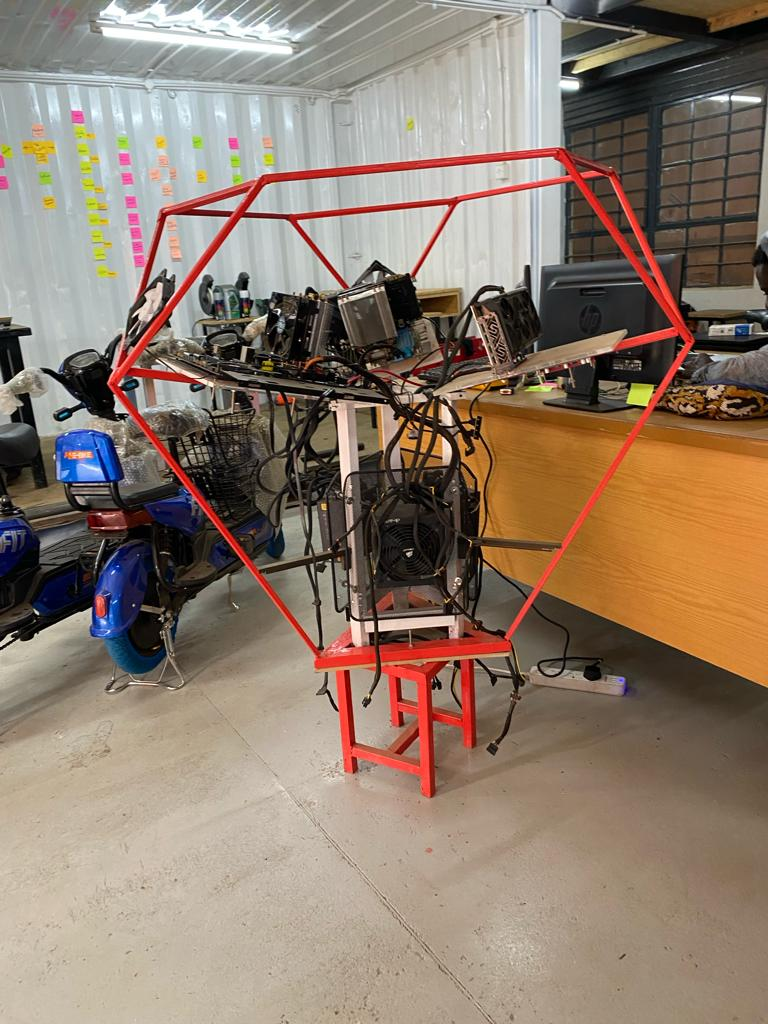
\includegraphics[width=0.8\textwidth]{images/gaming-server.jpeg}
    \caption{Gaming Server with Dual GPUs, Dual Motherboards, and Dual Power Supplies}
    \label{fig:Gaming Server with Dual GPUs, Dual Motherboards, and Dual Power Supplies}
\end{figure}